\documentclass[12pt, letterpaper]{article}
\usepackage[utf8]{inputenc}

\usepackage{geometry}
\geometry{
a4paper,
left=25mm,
right=25mm,
top=25mm,
bottom=25mm
}

% TODO: Do I want 1 or 2 columns?
\usepackage{multicol}

\usepackage{graphicx}
\graphicspath{ {images/} }
\usepackage{wrapfig}

\usepackage{textcomp}

\usepackage{hyperref}
\usepackage[all]{hypcap}

% Set the link style for the document.
\hypersetup{
colorlinks,
citecolor=blue,
filecolor=blue,
linkcolor=blue,
urlcolor=blue
}

\usepackage[explicit]{titlesec}

\titleformat{\paragraph}[runin]
{\normalfont\normalsize\bfseries}{\theparagraph}{1em}{#1\quad--}


% Start fix titlesec numbering.
\usepackage{etoolbox}
\makeatletter
\patchcmd{\ttlh@hang}{\parindent\z@}{\parindent\z@\leavevmode}{}{}
\patchcmd{\ttlh@hang}{\noindent}{}{}{}
\makeatother
% End fix titlesec numbering.


\providecommand{\keywords}[1]{\textbf{\textit{Keywords---}} #1}

% ==============================================================================



\title{Spectrangle}
\author{Wybe Westra --- s1578472}
\date{Software Systems \\ \today}

\begin{document}

    \maketitle

    \newpage

    \tableofcontents

    \newpage


    \section{Design}

    Spectrangle is implemented using a separate server and client.
    The game functionality is divided between the two according to the requirements laid out in the module manual,
    with one small exception.
    One cannot select a port for the server or client.
    This is because the network protocol determines that only port 4000 is to be used.

    Other than that, all the functionality required for single-person ``groups'' is implemented.

    % ------------------------------------------------------------------------------------------------------------------

    \subsection{Client and MVC}

    \begin{figure}[ht]
        \begin{center}
            \includegraphics[width=\textwidth]{Client.png}
            \caption{Diagram depicting how the client functions.
            Red blocks are separate threads.}
            \label{fig:clientDiagram}
        \end{center}
    \end{figure}

    The client is designed using the Model-View-Controller pattern.
    As visible in~\autoref{fig:clientDiagram}, the classes are named according to their role.
    The ClientController fulfills the Controller role, the GameModel is the model,
    and the TuiView is a view that uses the terminal to communicate with the user.

    The GameModel only exists when there is a game ongoing.
    Outside of a game, the GameModel reference points to `null`.

    Also laid out in~\autoref{fig:clientDiagram} are the two threads that the client uses during runtime.
    The Network thread is responsible for receiving and parsing the messages received from the server.
    When a valid message is received, it calls the appropriate method on the ClientController.
    The controller then either updates the model, or directly calls a method on the view.
    The only times the controller directly calls the view, is outside of a game or when a chat message arrives.
    The chat message bypasses the GameModel because it is not really part of the game.

    The input thread is continuously reading from the TUI .
    The main reason it is done like this, instead of polling the user when input is needed, is to facilitate the chat
    mechanism.
    The program has no idea when the user might want to send a chat message, so it needs to continuously read the input.
    Doing this, and listening to the server at the same time necessitates two threads.
    It has the nice side-effect that it allows the user to also input other commands at any time.
    For example, one could input `exit` while being asked for what tile to place, and it would parse just fine.
    After the input thread parses the command, the appropriate method on the controller is called.

    The only state held by the view is the current prompt for the user, and the chat history.
    The rest of the state, including things like which move the user wants to make, is kept in the GameModel.

    The GameModel is implemented as an observable, and is observed by the view.
    When the GameModel is updated by the network thread, or the input thread, it notify's the observers, which in this
    case is only the view.
    The notification includes a reference to the GameModel itself, along with a GameModel.Change enum, that signals
    what kind of update this is.
    The view takes this update, and changes it's prompt to the user according to the current state of the GameModel.
    For example, if the GameModel notifies the view that the player should select a tile to place, the view will
    update it's prompt to reflect that.

    The GameModel contains several self-defined classes, some of which are shared with the server.
    A diagram of the GameModel and the classes it contains as fields, can be seen in~\autoref{fig:modelDiagram}.
    The functionality and storage formats used by these classes
    will be further elaborated in~\autoref{subsec:Descriptions}.

    % TODO: A clear description of formats for data storage and communication. For communication use the design pictures.

    % ------------------------------------------------------------------------------------------------------------------

    \subsection{Server}

    \begin{figure}[ht]
        \begin{center}
            \includegraphics[width=\textwidth]{Server.png}
            \caption{Diagram depicting how the server functions.
            Red blocks are separate threads.}
            \label{fig:serverDiagram}
        \end{center}
    \end{figure}

    The server utilizes significantly more threads as the client.
    This can be seen in~\autoref{fig:serverDiagram}, where each red block represents a separate thread.

    The first thread to start is the main thread, which then starts up the Lobby thread.
    The main thread monitors the server socket, and creates a new ClientPeer for every connecting client.
    It starts the client's thread and then hands of the client to the Lobby, via a synchronized variable.

    Each ClientPeer thread continuously listens for messages from it's client.
    It parses each message, and if necessary sets a variable that indicates the client wants to do something.
    For example, each client has a queue of chat messages that it received.
    The thread currently responsible for that client periodically empties the queue and passes them on.
    The thread that has the client can also send messages through this connection, either by sending a raw string
    or via methods that implement messages from the networking protocol.
    Each client prints out the messages that get sent or received, so that it is clear what is going on.

    The Lobby receives new clients from the main thread and puts them in the waiting list.
    It periodically checks on the clients in this list, to see if they have requested a game, or if they have
    sent a chat message.
    There is a separate lobby list for each possible amount of players in a game, so 2, 3 and 4.
    The clients are placed in these lists after they have requested a game with the corresponding amount of players.
    Each list of players can only chat with the players in that list.

    After there are enough players, the Lobby starts a new Game.
    Each Game runs in a separate thread, so that two games won't step on each others toes
    and have to wait for each other.
    The Game enforces the rules, and keeps track of the tile bag, the Board, turn order, scores and other game
    related things.
    Details on how these are stored can be forund in~\autoref{subsec:Descriptions}
    When a game finishes, the Lobby takes back the clients and puts them back into the waiting list.

    % ------------------------------------------------------------------------------------------------------------------

    \subsection{Class descriptions}
    \label{subsec:Descriptions}

    % TODO intro.

    % TODO: For each self-defined class:
    %– The responsibilities of the class in the system. I.e., which functional requirements does it im-
    %plement? If applicable, which rule(s) does it implement? Which role does it play in the imple-
    %mentation of the Model-View-Controller or Observer pattern (if any)?
    %– For all classes that it refers to (i.e., as a field type, super type, argument type, local variable type
    %or by calling its constructor) you should describe the purpose of using this class.

    % TODO: A clear description of formats for data storage and communication. For communication use the design pictures.

    % ------------------------------------------------------------------------------------------------------------------

    \subsubsection{Game pieces}

    All the shared classes that are related to a game of Spectrangle.

    \paragraph{Abstract: AbstractPlayer}

    \paragraph{Board}

    \paragraph{BoardCoordinates}

    \paragraph{BoardSpace}

    \paragraph{Move}


    \paragraph{Tile}

    \paragraph{Enum: Color}

    \paragraph{Interface: TileBag}

    \paragraph{RandomTileBag}


    \paragraph{EmptyTileBagException}
    This exception get's thrown by a TileBag when takeTile is called when the bag is empty.

    \paragraph{IndexException}
    This get's thrown by methods of Board and BoardCoordinates, either when a function is called with invalid
    coordinates, or when a function that returns coordinates can't return valid ones.

    \paragraph{InvalidMoveException}
    Thrown by the Boards makeMove method when the move is not a valid one.

    \paragraph{NoTileException}
    Thrown by the Boards getTile method when the space at the given id does not have a tile.

    % ------------------------------------------------------------------------------------------------------------------

    \subsubsection{Networking}

    All the shared classes related to the network communication.
    Both the client and the server have their own implementation of the AbstactPeer.

    \paragraph{Abstract: AbstractPeer}

    \paragraph{Interface: Connection}

    \paragraph{SocketConnection}

    \paragraph{DeadConnectionException}
    Thrown by Connections when a readMessage or sendMessage is attempted, and the connection is broken.

    \paragraph{DecodeException}
    Thrown by Color and Tile when the message passed to their decode methods fails to parse.

    \paragraph{InvalidCommandException}
    Thrown by the message parsing methods of the ServerPeer and ClientPeer classes.
    Indicates that the message given does not translate to a valid command.
    Usually leads to this error being printed, and an `invalidCommand' message being sent over the Connection.


    % ------------------------------------------------------------------------------------------------------------------

    \subsubsection{Client classes}

    These classes are exclusive to the client.

    \paragraph{Client}

    \paragraph{ClientController}

    \paragraph{GameModel}

    \paragraph{Player}

    \paragraph{ServerPeer}

    \paragraph{Interface: SpecView}

    \paragraph{TuiView}

    \paragraph{SpectrangleBoardPrinter}
    Helper class to convert a spectrangle board into an understandable string that can be printed onto the TUI .

    The getBoardString method requires 4 lists of exactly 36 elements to function properly.

    \paragraph{GameStartedWithoutUsException}
    Thrown by the ClientController when the ServerPeer calls the startGame method, but the
    players listed in that game do not include this client.

    \paragraph{InvalidNumberException}
    Thrown by the ClientController when the view calls a method that requires the user to input a number, and
    the given number is not within the expected range.

    \paragraph{NoSuchPlayerException}
    Thrown by the ClientController and the GameModel when the ServerPeer calls a method that requires a player name,
    but there is no player with that name participating in the game.


    % ------------------------------------------------------------------------------------------------------------------

    \subsubsection{Server classes}

    These classes are exclusive to the server.

    % TODO: For each of the three most complex server classes:
    %– Which precautions must be taken to fulfill the preconditions in the contract of the class.

    \paragraph{Server}

    \paragraph{Lobby}

    \paragraph{Game}

    \paragraph{Player}
    % TODO how does this one differ from the client player.

    \paragraph{ClientPeer}

    % ------------------------------------------------------------------------------------------------------------------

    \section{Testing}
    \label{sec:testing}
    % TODO: Test report

    % TODO optonal: Unit tests. Some of these are not really Unit tests. More function or integration tests?
    %                  You have a nice reference that explains how each test is called in your QOWnnotes thing.

    % TODO optional: A report of the unit tests for each of the three most complex server classes:
    %– Besides the class under test, which other self-defined classes are executed during each test.
    %– The expected results for each test together with an explanation of the expected result (e.g., refer
    %to the game rules or functional requirements), as well as the actual result when running the test.
    %– A discussion of the test coverage of the class under test. Explain whether you consider the
    %reached level of coverage high or low. For those parts of the code that are not covered, you
    %should also discuss why they are not covered (e.g., why was it difficult to write tests that cover
    %them).

    % TODO: SYSTEM tests.

    % ------------------------------------------------------------------------------------------------------------------

    \subsection{Test classes}
    \label{subsec:testClasses}

    These are classes that implement the interfaces defined in the program in such a way that the input and output can
    be controlled.
    This is mostly done in cases where the normal implementation uses network access, or involves non-deterministic
    behaviour.
    Instances of these classes can then be passed to an object that is being tested, so that all conditions are known
    beforehand.

    \paragraph{MockTileBag}
    This tile bag works exactly like the RandomTileBag, except it isn't random.
    The starting tiles are added in a pre-determined order, and will be drawn from the bag in the same order.
    This way, when it is passed to a Game class, it is known upfront what tiles the players are going to draw.
    Using this the rules of the game can be reliably tested, in a way that will fail or succeed in a deterministic
    fashion.

    \paragraph{MockConnection}
    This is an implementation of the Connection interface that doesn't depend on a Socket.
    Instead it has an internal list of messages that, for users of the interface, appear to be ``received'' or ``sent''.
    It implements some additional methods to allow unit tests to manipulate the message lists.
    This way the ServerPeer and ClientPeer can both be tested as if they had a connection, without actually requiring
    any I/O.

    % ------------------------------------------------------------------------------------------------------------------

    \section{Planning}
    \label{sec:planning}

    First off, I did not do the design project, so there are no influences of that in here.

    The original plan was to do the design of the program in the first few days.
    Then the implementation of the rules from the 14th of Januari to the 18th.
    After that, the networking should be ready a the 23th and we could build the AI till the 26th.
    This would give us 4 days to do the final touches on the report.

    This went okay for the designing of the program, but from then on it quickly devolved.
    Once again it turns out that it's one thing to make a plan, and another to stick with it.
    On top of that, the original plan wouldn't have worked in the first place, as we understood
    ``implementing the rules'' to be ``create a single player version''.
    And then the idea was that we could add in the networking where necessary.
    That was never going to work, as the networking is a really integral part of the program.
    Trying to shoehorn it in after creating a single player version would be really unwieldy.

    So we didn't do it that way.
    Or at least, I didn't.
    While I normally don't want to bash on teammates, it was mostly me doing the programming during the majority of the
    project.
    Me programming on the premise that it was a two people project meant that progress didn't go as fast as it should.
    So in the end, when my project partner ended up stopping the module and I became an official one-person ``group'',
    the extension was very welcome.
    It's also why I am writing this on the last day before submission.

    Next time I will be much more proactive in getting team-mates to pull their weight.
    Also, I now know that the networking part of a networked program is not something you can add halfway through.
    Instead you have to design the progrma with it in mind from the get-go, and adjust your planning accordingly.

    \begin{figure}[t]
        \begin{center}
            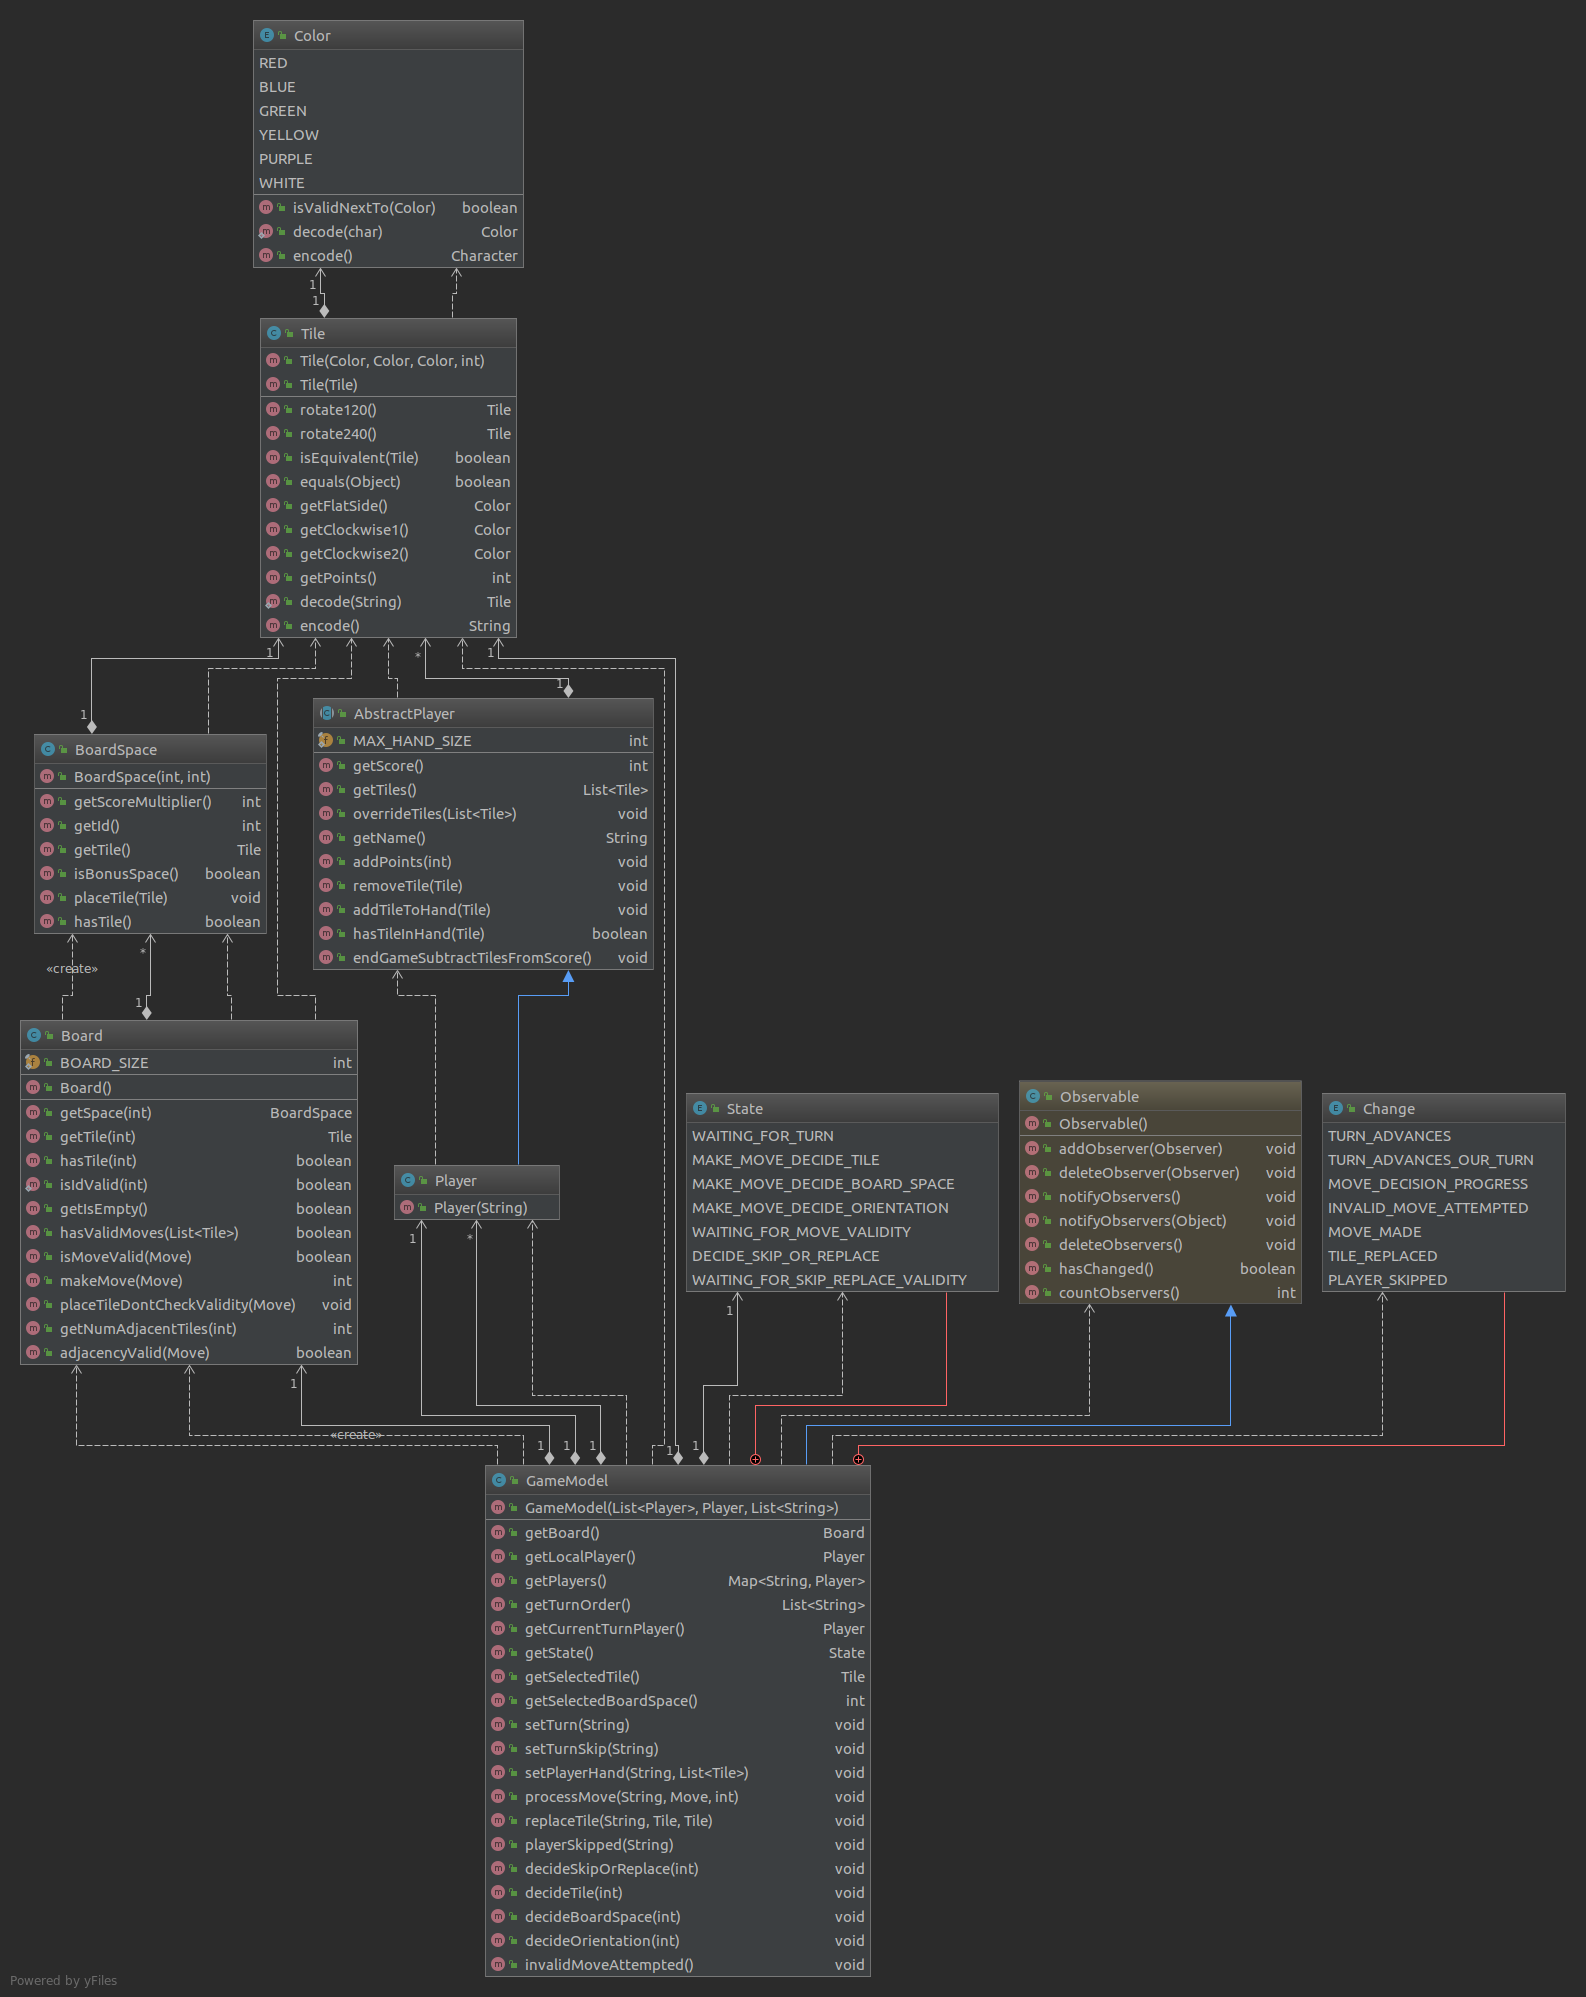
\includegraphics[width=\textwidth]{GameModel.png}
            \caption{Class diagram of the GameModel and the other self-defined classes it contains.}
            \label{fig:modelDiagram}
        \end{center}
    \end{figure}


\end{document}
